
\section{Rappels}

\begin{frame} \frametitle{Le modèle de données Cassandra}

  Cassandra organise les données en \alert{tables} dénormalisées

  \vfill

  Principales différences avec le modèle relationnel

  \vfill
  \begin{redbullet}
  \item Pas de clé étrangère (et pas de jointure)
  \item Imbrication (\textit{nesting}) de valeurs structurées
  \item Pas d'indépendance logique/physique\,: la clé
      détermine le placement
   \item Sauf exception, les recherches se font sur la clé
  \end{redbullet}

  \vfill

  \begin{defblock}{Principe de conception}
  Pas de jointure, donc pas de symétrie d'accès\,: on doit organiser
  les données en fonction des accès applicatifs.

  \end{defblock}
\end{frame}


\begin{frame}[fragile]
\frametitle{Imbrication de structures}

C'est le principe de dénormalisation\,: on regroupe 
les données le plus possible dans des lignes pour éviter les jointures.

\vfill

Une valeur d'attribut  peut correspondre\,:
\begin{redbullet}
	\item à un ensemble de valeurs (non ordonnées)\,: \textbf{SET} 
	\item à une liste de valeurs\,: \textbf{LIST}
	\item à un dictionnaire\,: \textbf{MAP} 
	\item à un nuplet\,: \textbf{TUPLE} 
	\item à une instance d'un type utilisateur
\end{redbullet}

\vfill

Les ensembles doivent rester de taille raisonnable
\end{frame}


%%%%%%%%%%%
\begin{frame}[fragile] \frametitle{Principes de conception}

On adopte un des nombreux schémas possibles en 
fonction des besoins.

\vfill

\begin{redbullet}
		\item On conçoit les \alert{chemins d'accès}, ou séquence des requêtes émises par une application
		
		\item On organise les tables pour que  chaque requête  s'exécute \alert{localement} et \alert{séquentiellement}
		
		\item On peut créer ponctuellement des index ou des vues matérialisées
		
		\item Au pire (mais inévitable\,?) on multiplie les organisations physiques et donc la redondance
	\end{redbullet}

\vfill

\begin{defblock}{Pour quelle type d'application\,?}
Acceptable pour une approche WORM (\textit{Write Once, Read many})
\end{defblock}
\end{frame}

%%%%%%%%%%%%%%
\begin{frame}[fragile]{Notre modèle}

\begin{center}
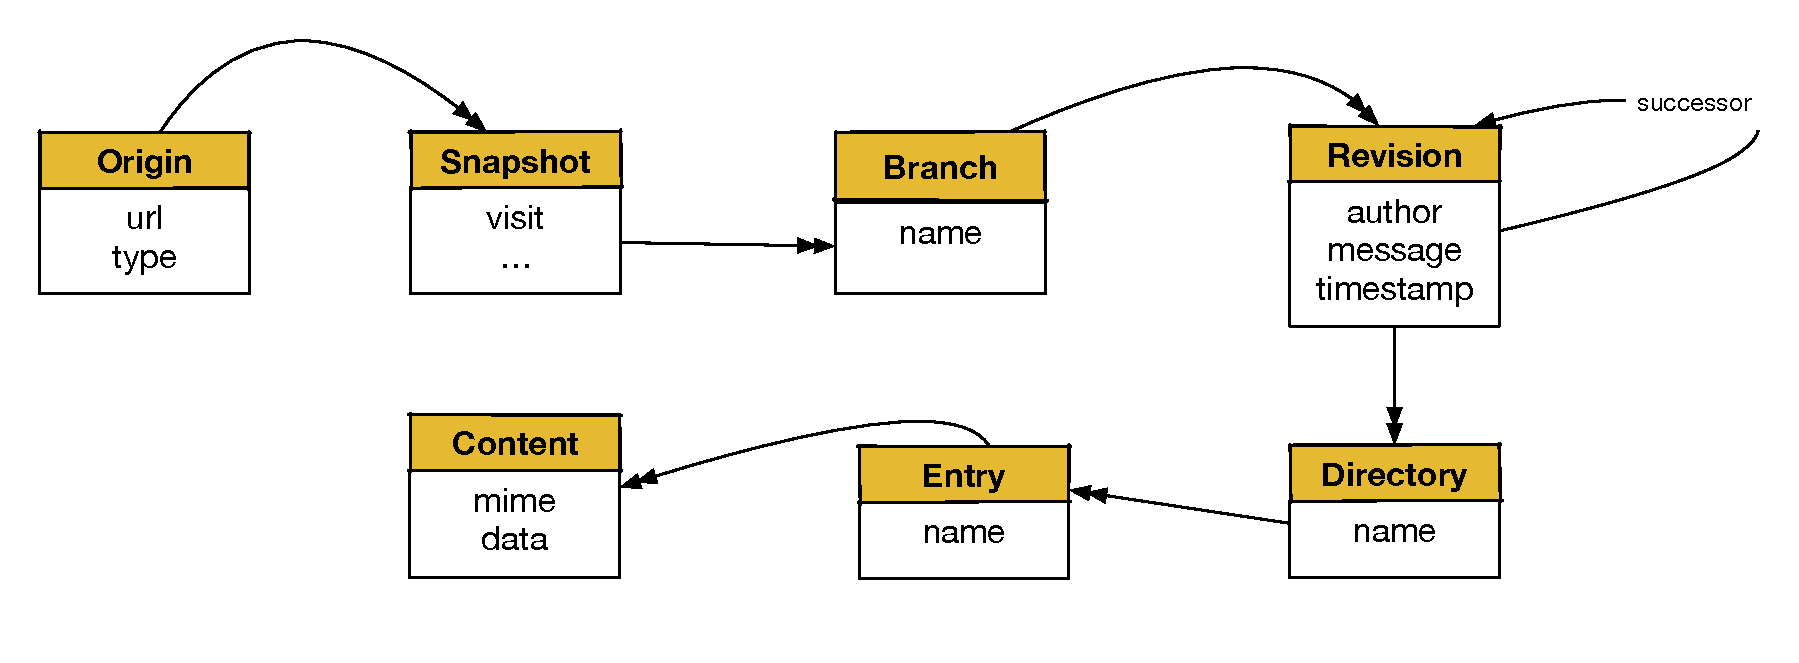
\includegraphics[width=\textwidth]{../figures/modele_swh.pdf}
\end{center}

Pour chaque table on a un point d'accès (pe \texttt{'repository'}) et l'identification
relative à ce point d'accès (pe \texttt{'snapshot'}). On nommera la table 
\texttt{snapshot\_by\_repository}
\end{frame}


%%%%%%%%%%%%%
\begin{frame}[fragile] \frametitle{Quelques exemples\,: cherchons les visites}

Une première approche purement relationnelle ne fonctionne pas.
\vfill

\begin{columns}
    \begin{column}{0.45\textwidth}
    \alert{Schéma}
    \end{column}
        \begin{column}{0.45\textwidth}
    \alert{Requêtes}
    \end{column}
\end{columns}

\begin{columns}
    \begin{column}{0.45\textwidth}
  \begin{minted}{sql}
  create table Repository 
     (Repository_id uuid,
      url varchar, 
      description text,
      primary key (Repository_id))
  \end{minted}
  
  \begin{minted}{sql}
  create table Visit 
     (visit_id uuid,
      Repository_id
      visit_ref int,
      date date,
       primary key (visit_id) )
  \end{minted}
  \end{column}
 \begin{column}{0.45\textwidth}
  Il faut deux requêtes (pas de jointure)
  \vfill
  \begin{minted}{sql}
  select Repository_id in oid 
  from Repository 
  where url ='github.org/cassandra'
  \end{minted}

  \begin{minted}{sql}
  select * from Visit 
  where Repository_id = oid
  \end{minted}
  \vfill
  Et Cassandra refuse les deux ! 
\end{column}
\end{columns}

\end{frame}


%%%%%%%%%%%%%
\begin{frame}[fragile] \frametitle{Organisons les clés et chemins d'accès}

Les critères de recherche doivent impliquer la clé

\vfill
\begin{columns}
    \begin{column}{0.45\textwidth}
  \begin{minted}{sql}
  create table Repository 
     (url varchar, 
      description text,
      primary key (url)
      )
  \end{minted}
  
  \begin{minted}{sql}
  create table Visit_by_Repository
     (url_Repository varchar,
      visit_ref int,
      date date,
      primary key (url_Repository, 
                   visit_ref)
      )
  \end{minted}
  \end{column}
 \begin{column}{0.45\textwidth}

  \begin{minted}{sql}
  select * from Repository 
  where  url ='github.org/cassandra'
  \end{minted}
  
  \vfill
    \begin{minted}{sql}
  select * from Visit_by_Repository 
  where  url ='github.org/cassandra'
  \end{minted}
    \vfill
   
  \begin{minted}{sql}
  select * from Visit_by_Repository 
  where  url ='github.org/cassandra'
  and visit_ref < 3
  \end{minted}
    
\end{column}
\end{columns}

\end{frame}

%%%%%%%%%%%%%
\begin{frame}[fragile] \frametitle{Imbriquons pour avoir moins de tables}

\vfill
\begin{columns}
    \begin{column}{0.45\textwidth}
    
    Un type \texttt{Visit}
    
  \begin{minted}{sql}
  create type Visit (
      number int,
      date_visit date)
  \end{minted}
    
    \vfill
    Imbriqué dans \texttt{Repository}
    \vfill
  \begin{minted}{sql}
  create table Repository 
     (url varchar, 
      description text,
      visites list<Visit>,
      primary key (url)
      )
  \end{minted}
  
  \vfill
  Suppose un nombre limité de visites.
   \end{column}
 \begin{column}{0.45\textwidth}
  Une requête localisée et unique pour trouver toutes les visites d'un dépôt.

  \begin{minted}{sql}
  select * from Repository 
  where  url ='github.org/cassandra'
  \end{minted}
  
  \vfill
  Les dépôts visités au moins 10 fois
  
   \begin{minted}{sql}
  select * from Repository 
  where  url ='github.org/cassandra'
  and count(visit.number) >= 10
  \end{minted}
  
\end{column}
\end{columns}
	
\end{frame}


%%%%%%%%%%%%%
\begin{frame}[fragile] \frametitle{Tentons une modélisation complète\,: \texttt{Snapshot}}


\begin{columns}
    \begin{column}{0.45\textwidth}
     
  \begin{minted}{sql}
  create type Repository (
      description int,
      other_infos text)
  \end{minted}
    
    \vfill
  \begin{minted}{sql}
  create table Snapshot_by_Repo
     (url varchar, 
      snapshot_date,
      snapshot_id uuid,
      Repository Repository,
      branches map<string, uuid>,
      primary key (url, 
                   snapshot_date)  
      )
  \end{minted}
  Avec peu de branches par snapshot
   \end{column}
 \begin{column}{0.45\textwidth}

  Tous les snapshots d'une Repository.
  
  \vfill
  
  \begin{minted}{sql}
  select * from Snapshot_by_Repo
  where  url ='github.org/cassandra'
  \end{minted}
  
   \vfill
   Snapshots après une date et contenant une branche \texttt{master}
   
 \begin{minted}{sql}
  select * from Snapshot_by_Repo
  where  url ='github.org/cassandra'
  and snapshot_date > '01-MARCH-2024'
  and branches contains key 'master'
  \end{minted}

\vfill 
  On obtient les id des snapshots et des branches
\end{column}
\end{columns}
	
\end{frame}
	
	
%%%%%%%%%%%%%
\begin{frame}[fragile] \frametitle{Connaissant une branche\,: les \texttt{Revision}s}


\begin{columns}
    \begin{column}{0.45\textwidth}
  On poursuit la même démarche. Cette fois on
  a affaire à un graphe. Pas facile à modéliser efficacement.
    
  \begin{minted}{sql}
  create table Revision_by_branch
     (branch_id uuid, 
      revision_id uuid,
      parents list<uuid>,
      author varchar,
      message varchar,
      tstamp date, 
      primary key (branch_id, 
       revision_id)
      )
  \end{minted}
  
  
   \end{column}
 \begin{column}{0.45\textwidth}
   Toutes les révisions d'une branche par Stefano.
  
  \begin{minted}{sql}
  select * from Revision_by_branch 
  where  branch_id ='bxyz'
  and author = 'Stefano'
  \end{minted}
  
   \vfill
    Les révisions dont un parent est la révision 'abcd'
   
 \begin{minted}{sql}
  select * from Revision_by_branch 
  where   branch_id ='bxyz'
  and parents contains 'abcd'
  \end{minted}

\vfill 
  On obtient les id des révisions d'une branche. 
  
\end{column}
\end{columns}
	
\end{frame}
	


%%%%%%%%%%%%%
\begin{frame}[fragile] \frametitle{Et si je veux naviguer dans le graphe\,?}

Les parents et ascendants de la révision 'lklklk'. 
On obtient d'abord la liste des parents avec la requête
   
 \begin{minted}{sql}
  select parents from Revision_by_branch 
  where   branch_id ='bxyz'
  and revision_id = 'lklklk'
  \end{minted}

\vfill 
  Puis il faut faire une requête pour \alert{chaque} parent
  
  
 \begin{minted}{sql}
 select parents from Revision_by_branch 
  where   branch_id ='bxyz'
  and revision_id = 'id_du_parent'
  \end{minted}
  
\vfill

On a peut-être intérêt à charger une bonne fois le graphe
dans l'application.
\end{frame}
	
	
%%%%%%%%%%%%%
\begin{frame}[fragile] \frametitle{En résumé (provisoire)}

En synthèse\,:

\begin{redbullet}

   \item La clé primaire détermine le stockage \emph{et} les requêtes possibles
   
     $\Rightarrow$ \alert{clé de partitionnement} = point d'accès, \alert{clé de regroupement} =
   identifiant relatif au point d'accès
  
  \item Il faut parfois ``retourner'' une clé primaire si on souhaite un accès 
     symétrique à une table existante      (cf. exemple \texttt{révision/Directory})
     
      $\Rightarrow$  automatisable avec une vue matérialisée (forte redondance)

   \item L'imbrication d'ensembles ou listes peut limiter le nombre d'étapes 
   
      $\Rightarrow$ leur taille doit être restreinte, cf. exemple des branches
   
\end{redbullet}
	
\end{frame}


\end{document}

\end{document}


	
%%%%%%%%%%%%%
\begin{frame}[fragile] \frametitle{Connaissant une \texttt{Revision}\,: les \texttt{Directory}}


\begin{columns}
    \begin{column}{0.45\textwidth}
    Idem, structure d'arbre (?), une requête
  par directory. Pas idéal\ldots
  
  \vfill
  
   \begin{minted}{sql}
  create table Directory_by_revision
     (revision_id uuid,
      directory_id uuid,
      children list<uuid>,
      parent_id uuid,
      primary key (revision_id,
          directory_id)
      )
  \end{minted}

   On peut naviguer parent/enfants, mais une requête à chaque fois
   \end{column}
 \begin{column}{0.45\textwidth}
     À l'inverse si je veux avoir la liste des révisions
     d'une directory, je dois inverser la clé\ldots
   \begin{minted}{sql}
  create table Revision_by_directory 
     (directory_id uuid,
      revision_id uuid,
      children list<uuid>,
      primary key (revision_id,
          directory_id)
      )
  \end{minted}
   \texttt{Revision\_by\_directory} peut être une \alert{vue matérialisée}
    
\end{column}
\end{columns}
	
\end{frame}

%%%%%%%%%%%%%
\begin{frame}[fragile] \frametitle{Connaissant une \texttt{Directory}\,: les \texttt{Entry}}


\begin{columns}
    \begin{column}{0.40\textwidth}
   
  \begin{minted}{sql}
  create table Entry_by_dir
     (directory_id uuid, 
      name varchar,
      access_rights varchar,
      content_ref varchar,
      primary key (directory_id, 
       name)
      )
  \end{minted}

\vfill
 NB\,: sans doute trop d'entrées par directory 
 pour les représenter par une liste imbriquée
  
   \end{column}
 \begin{column}{0.50\textwidth}
  
  Toutes les entrées d'une directory
  
  \begin{minted}{sql}
  select name from Entry_by_dir
  where directory_id = 'xyz'
  \end{minted}
  
   \vfill
   
   Une entrée \texttt{README.md}
 \begin{minted}{sql}
  select content_ref from Entry_by_dir
  where directory_id = 'xyz'
  and name = 'README.md'
  \end{minted}
 
\end{column}
\end{columns}
	
\end{frame}
	
	
	
	
\begin{frame}[fragile]{Clause $WHERE$}
\begin{itemize}
	\item \textbf{Clé primaire = valeur} : Le plus efficace
	\item \textbf{token(Clé primaire) $>$ valeur} : Liste de tokens par noeud
	\item \textbf{attribut = valeur} + \textbf{INDEX} : Moins efficace
	\item \textbf{attribut = valeur} + \textbf{ALLOW FILTERING} : Pas efficace\\test sur tous les noeuds
	\item \textbf{Données imbriquées} :
	\begin{itemize}
		\item \textsc{SET} : \textit{CONTAINS}
		\item \textsc{LIST} : \textit{CONTAINS}
		\item \textsc{MAP} : \textit{CONTAINS KEY}\\ou clé directement : hotesse.prenom = 'Natacha'\\
		Les clés peuvent être indexées
		\item \textsc{SubType} : att = valeur (tuple imbriquée = BLOB)
		\item[$\Rightarrow$] Le \textit{MAP} est à privilégier
	\end{itemize}
\end{itemize}
\end{frame}

\end{document}